\appendix
\renewcommand{\thesection}{APPENDIX \Alph{section}}
\section{ - Figures} \label{appendix:A}
\topskip0pt
\vspace*{\fill}
\begin{center}
    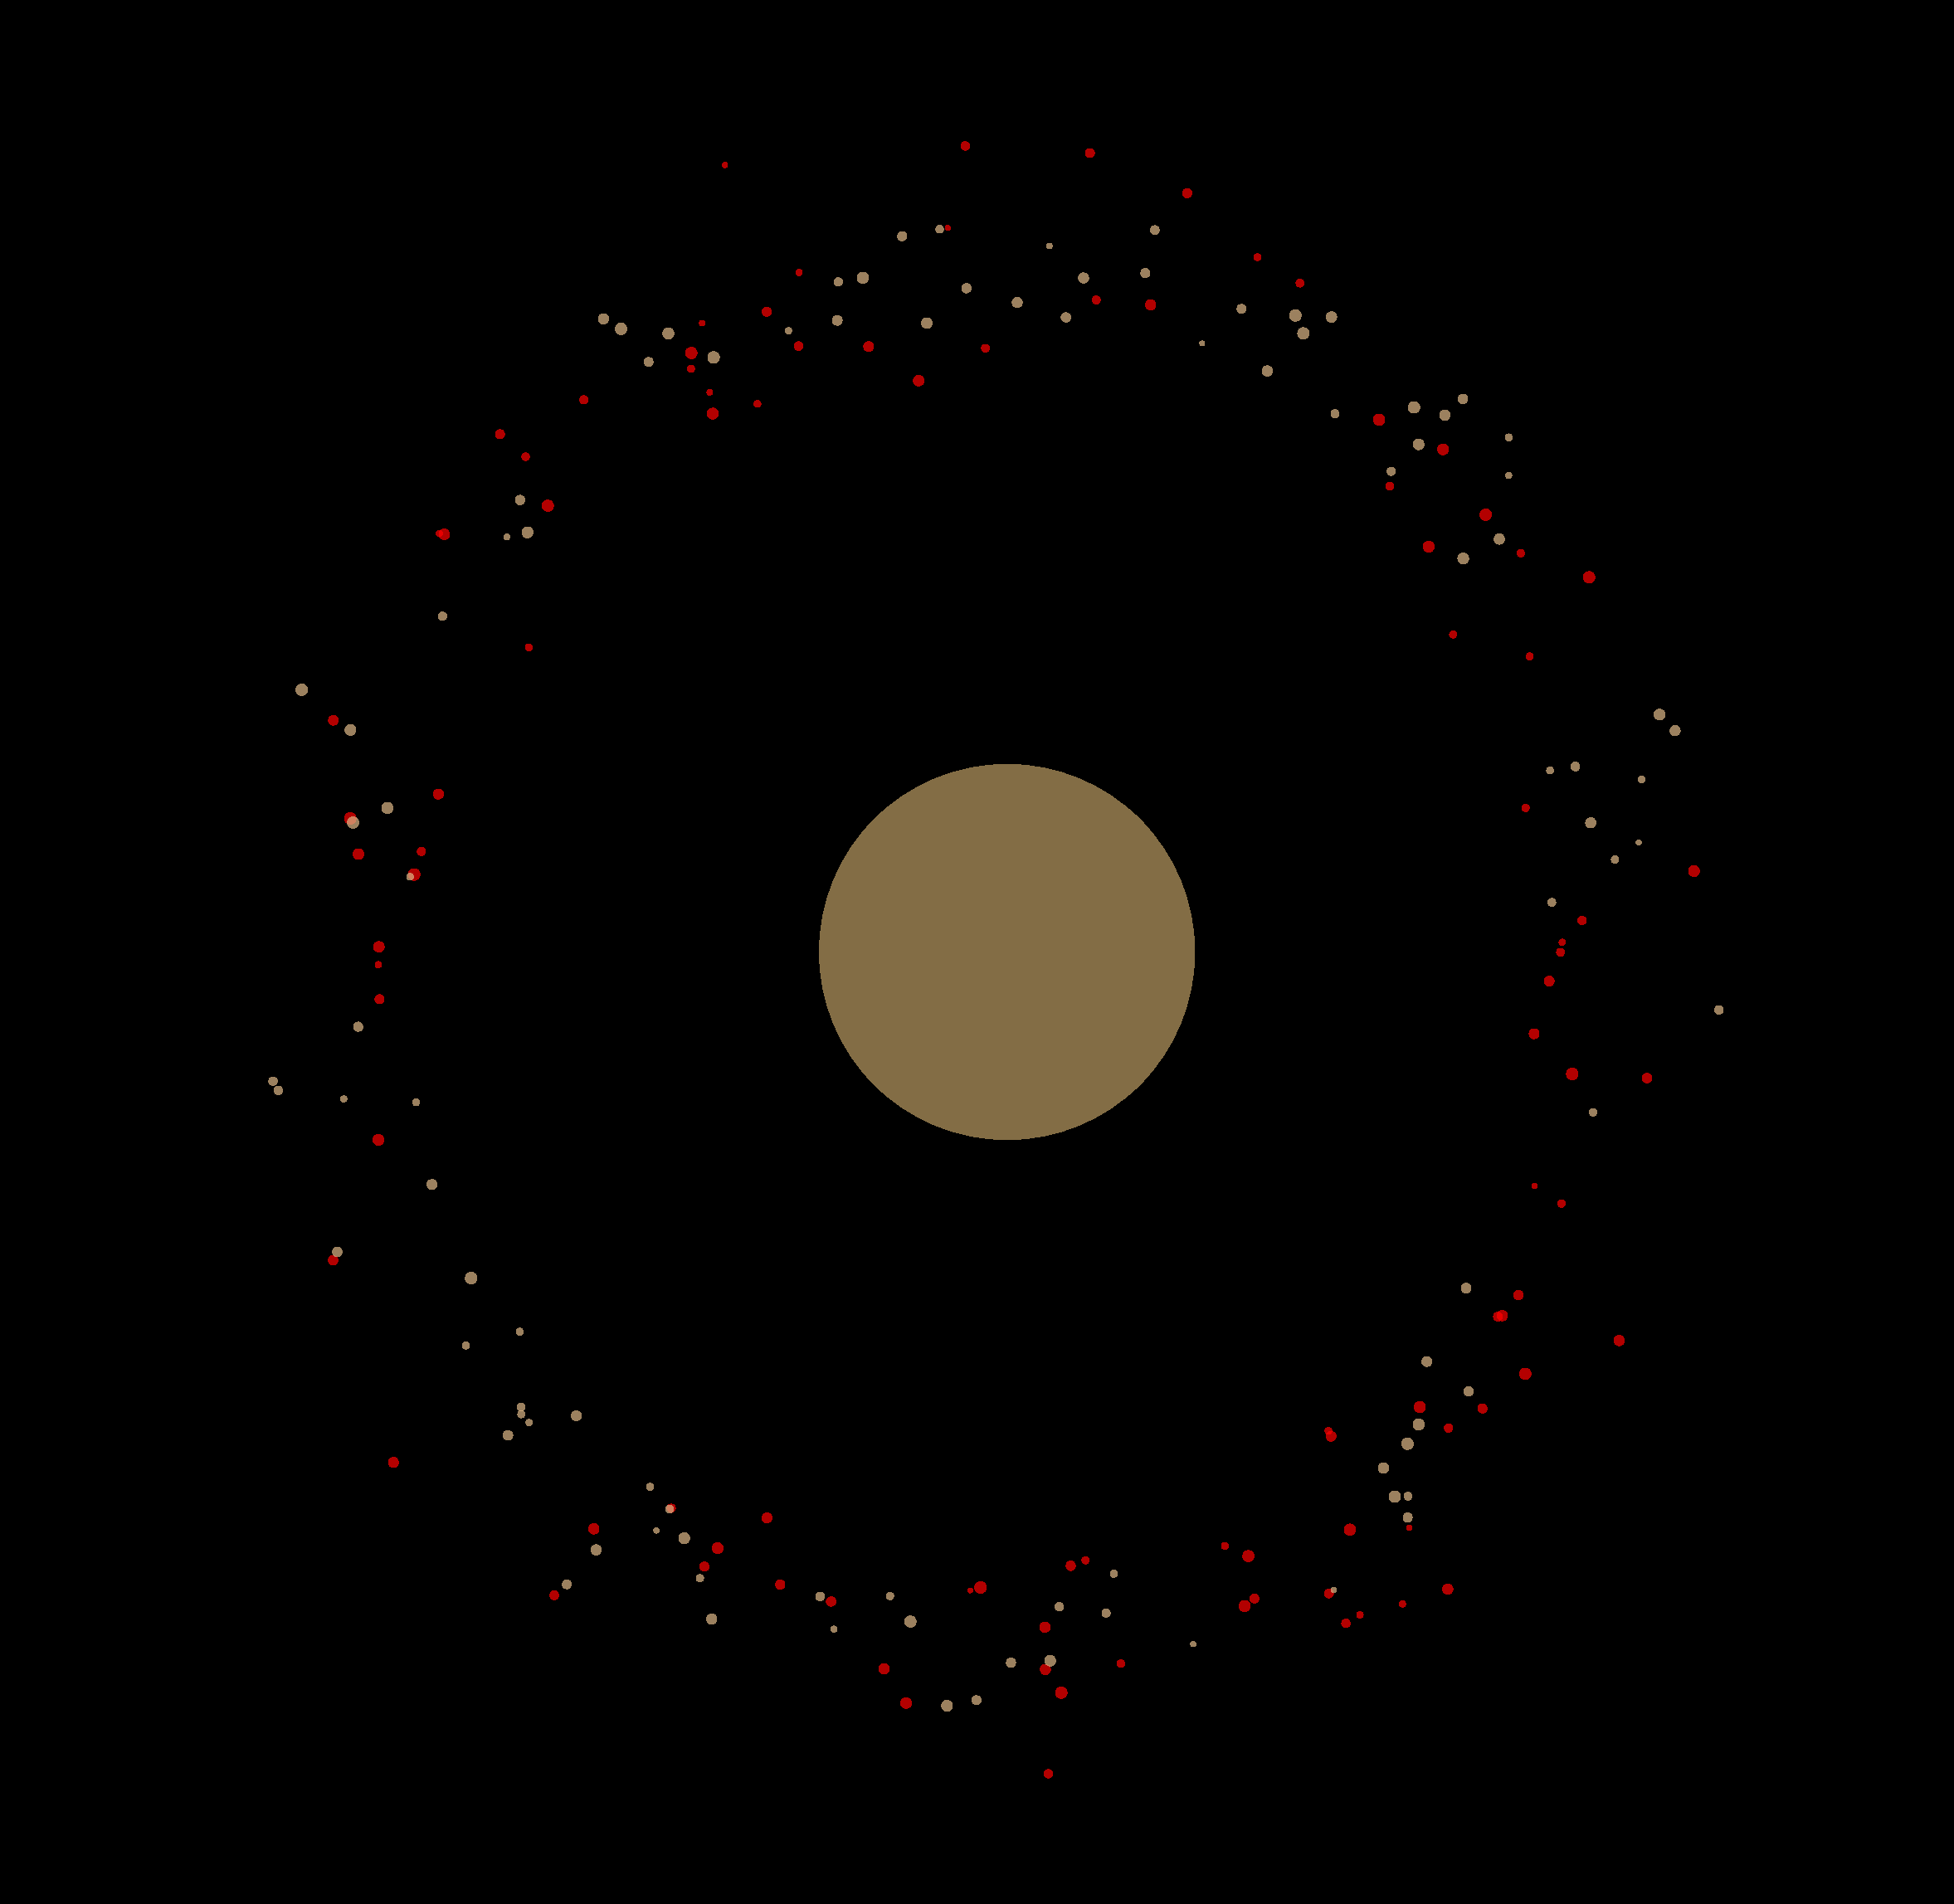
\includegraphics[width=\textwidth]{{img_src/scatter_final_max_10_y_dt_0.001_y}.pdf}
    \captionof{figure}{The starting and final positions of the asteroids with $dt = 0.001$ years and $t_{max} = 10$ years. The red dots indicates the final positions, while the burly wood color points are the starting locations.} \label{fig:4}
\end{center}
\vspace*{\fill}
\newpage
\topskip0pt
\vspace*{\fill}
\begin{center}
    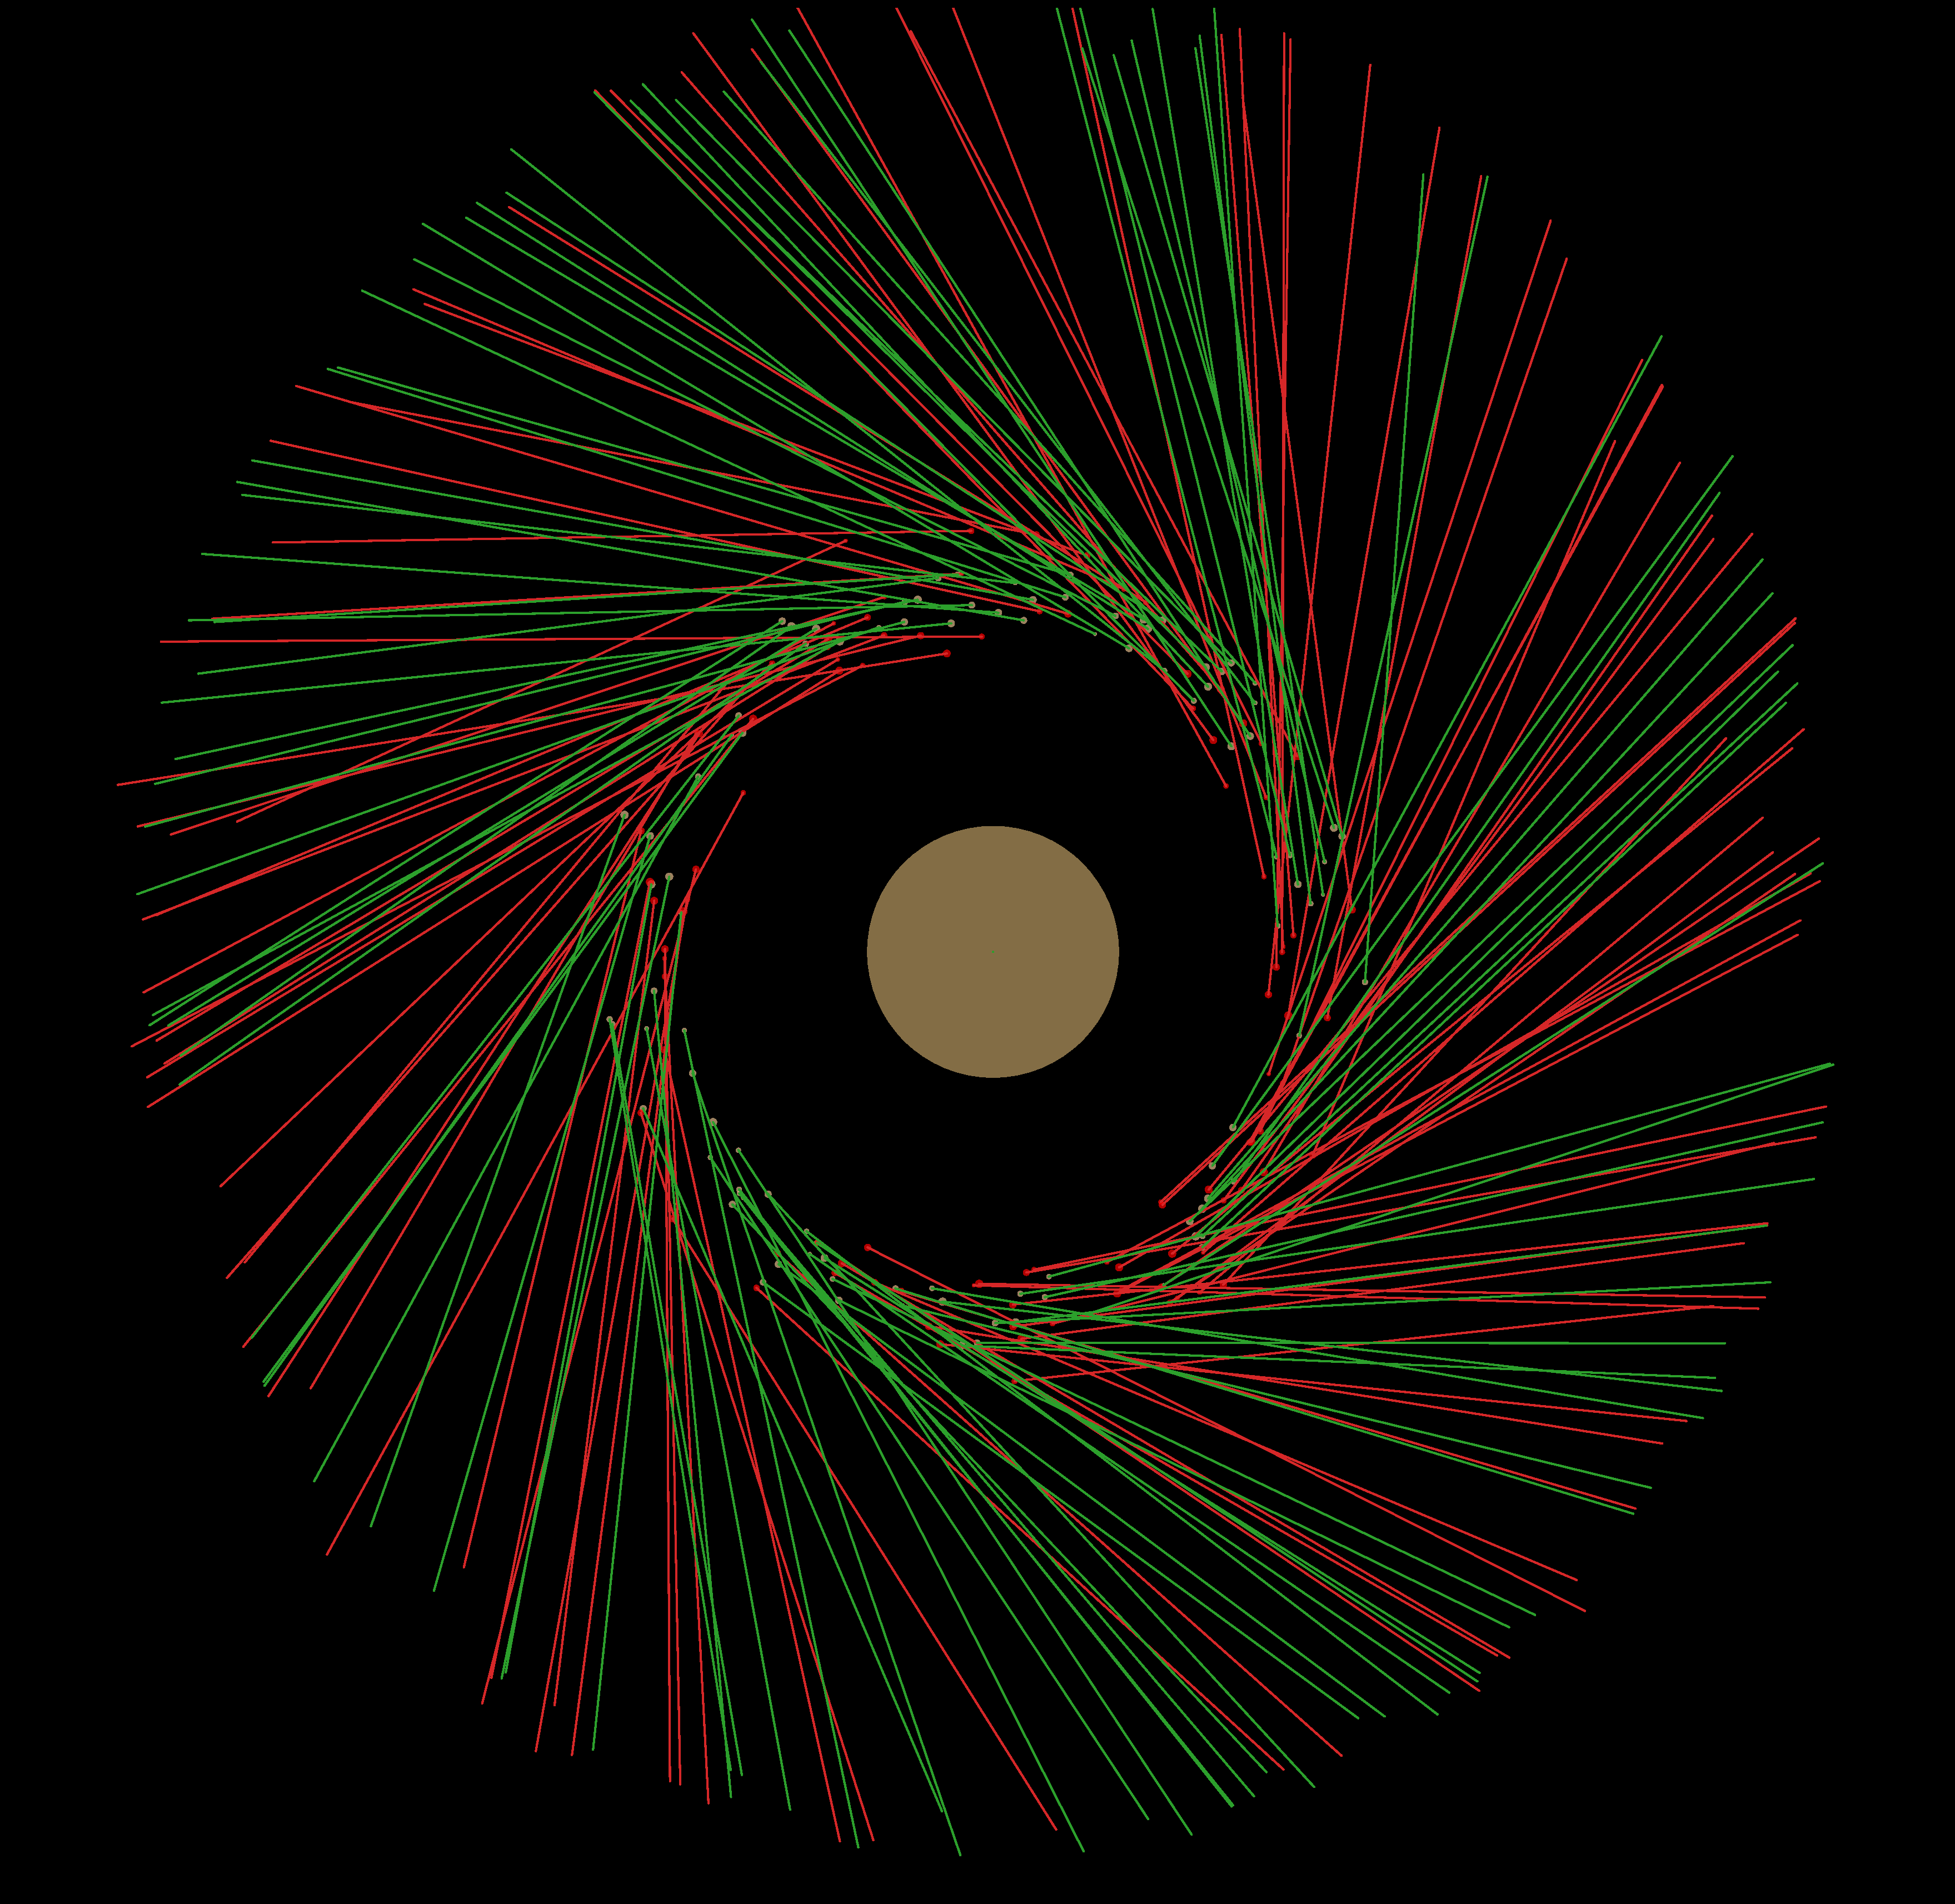
\includegraphics[width=\textwidth]{{img_src/velocity_final_max_10_y_dt_0.001_y}.pdf}
    \captionof{figure}{The starting and final positions and corresponding velocity vectors of the asteroids with $dt = 0.001$ years and $t_{max} = 10$ years. The red dots with red lines indicates the final positions and length of the velocity vectors, pointing into their actual directions, while the burly wood color points and green lines are the starting locations and length of the velocity vectors, pointing into the correct directions. The velocities are measured in AU y$^{-1}$ and they are shortened on the graph to the $\frac{100}{8760}$ of their original length.} \label{fig:5}
\end{center}
\vspace*{\fill}
\newpage
\topskip0pt
\vspace*{\fill}
\begin{center}
    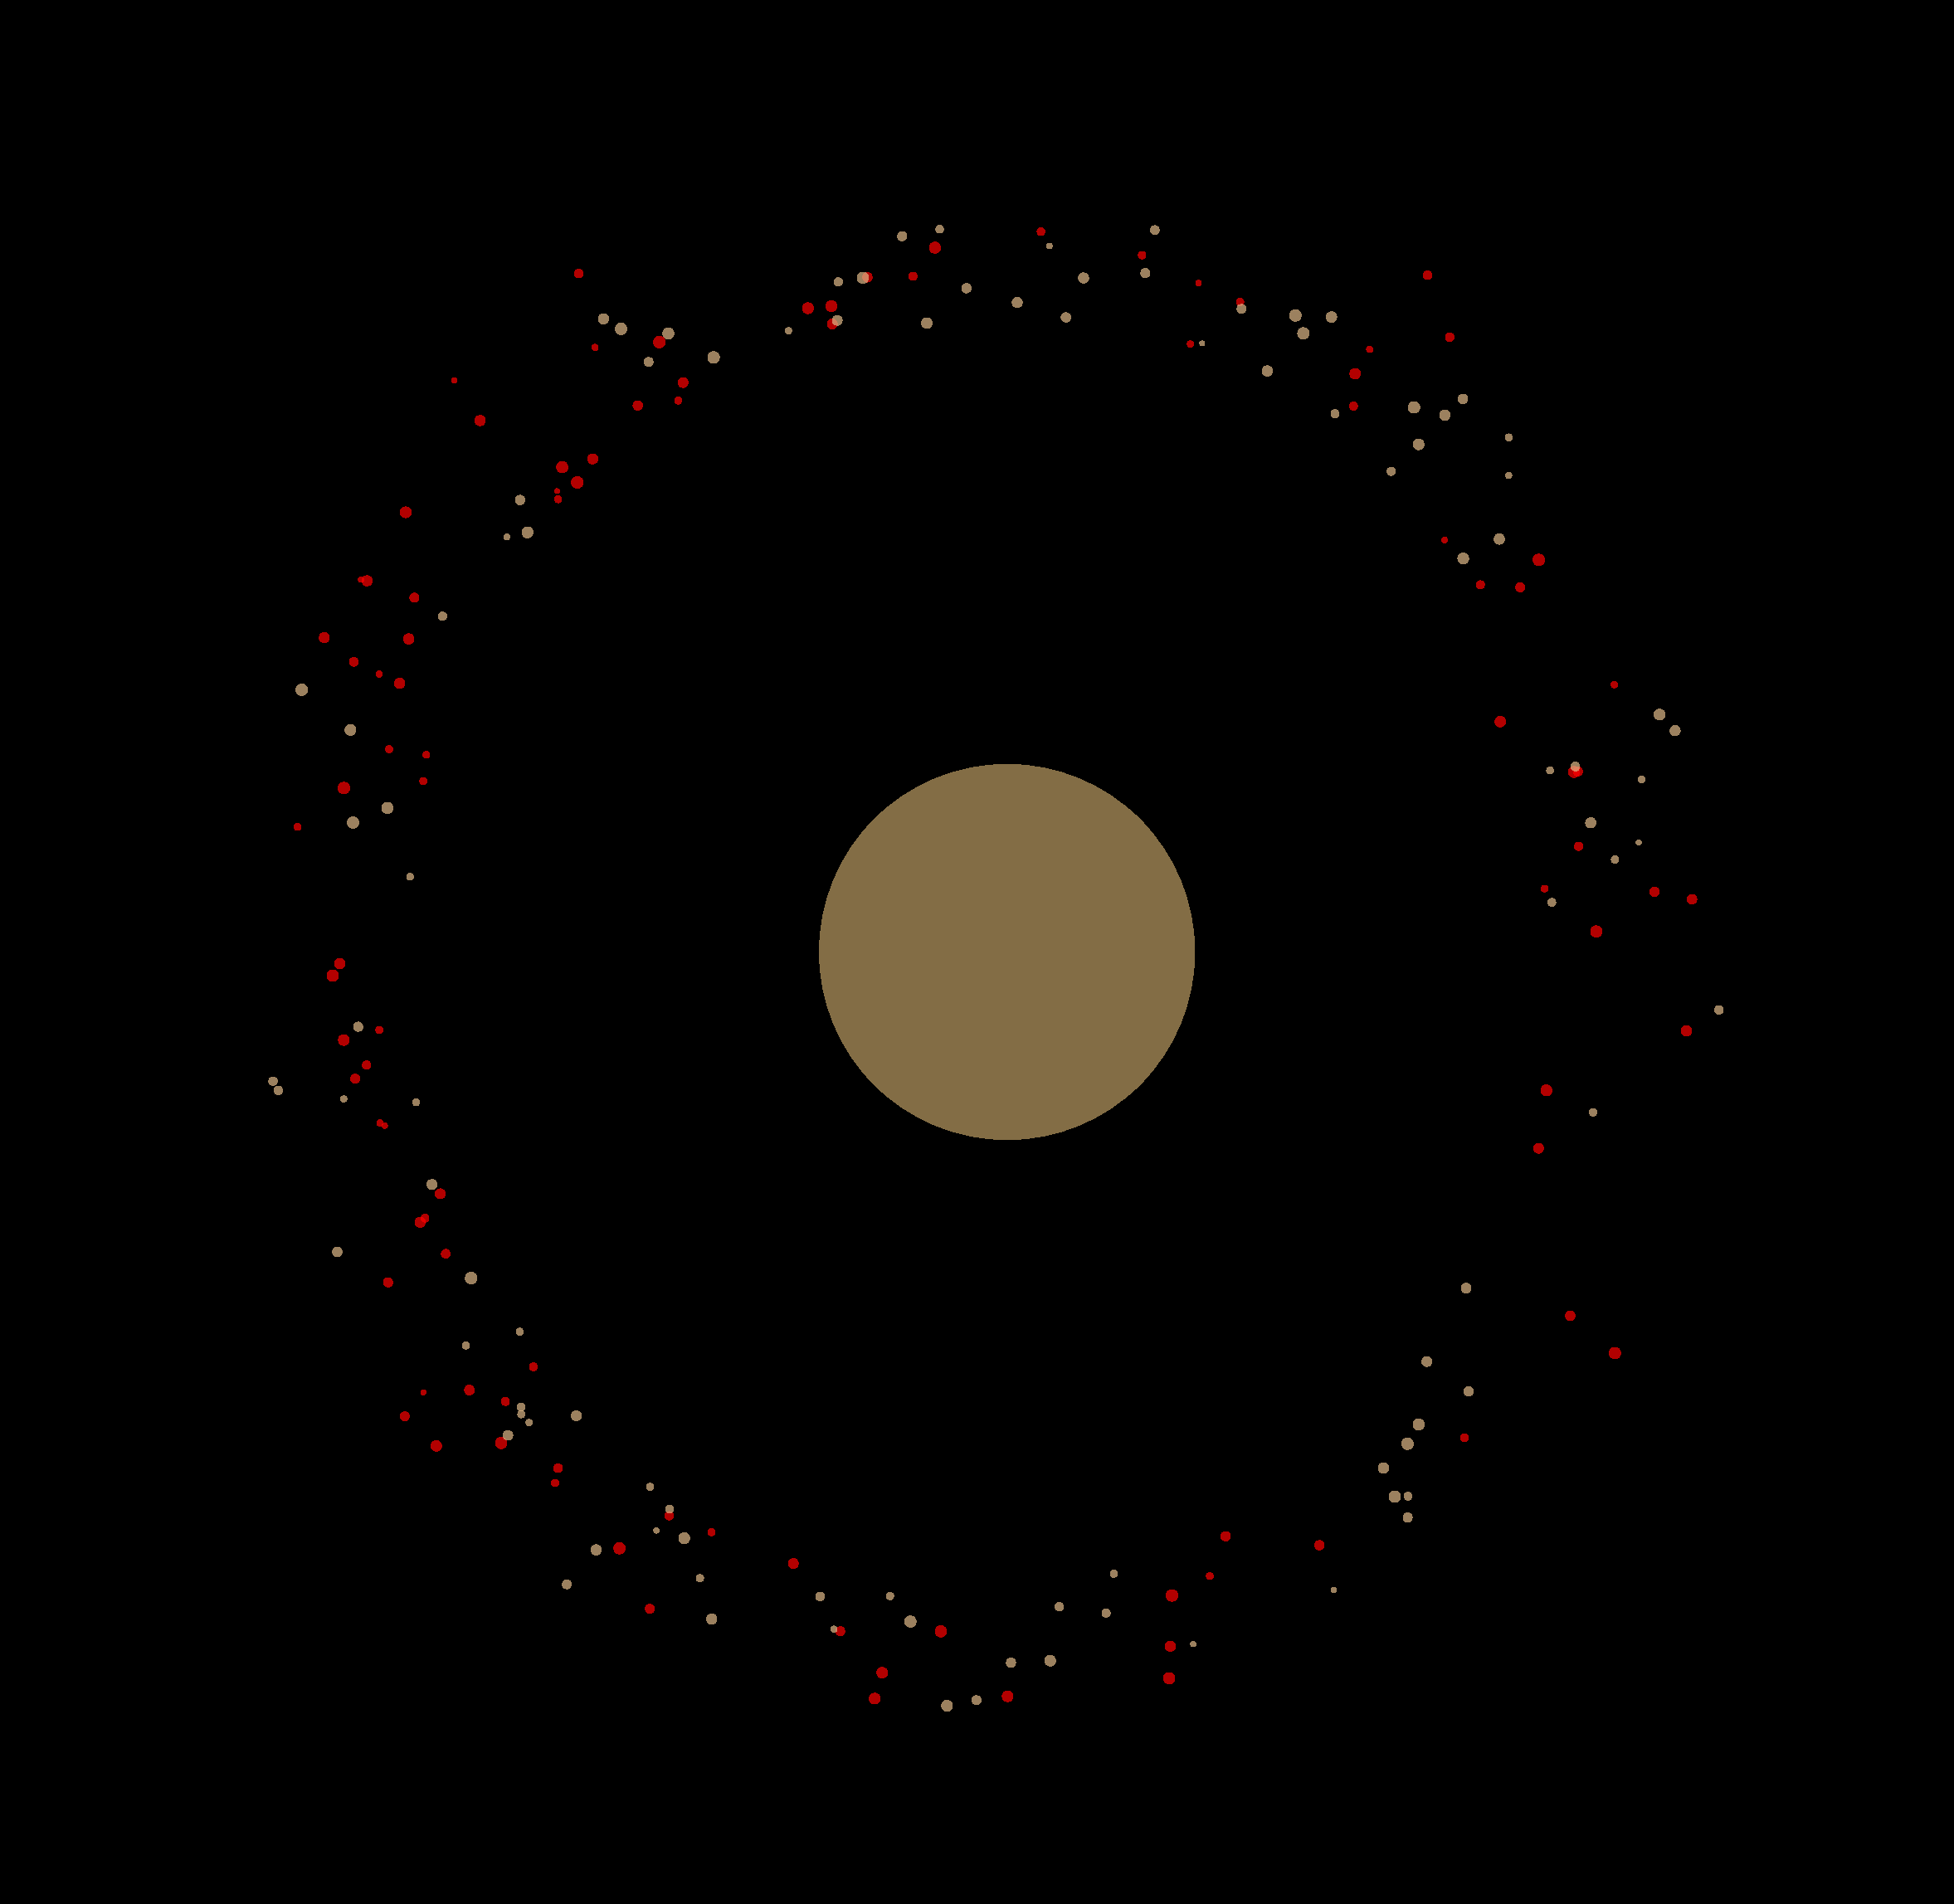
\includegraphics[width=\textwidth]{{img_src/scatter_final_max_100_y_dt_0.0001_y}.pdf}
    \captionof{figure}{The starting and final positions of the asteroids with $dt = 0.0001$ years and $t_{max} = 100$ years. The red dots indicates the final positions, while the burly wood color points are the starting locations.} \label{fig:6}
\end{center}
\vspace*{\fill}
\newpage
\topskip0pt
\vspace*{\fill}
\begin{center}
    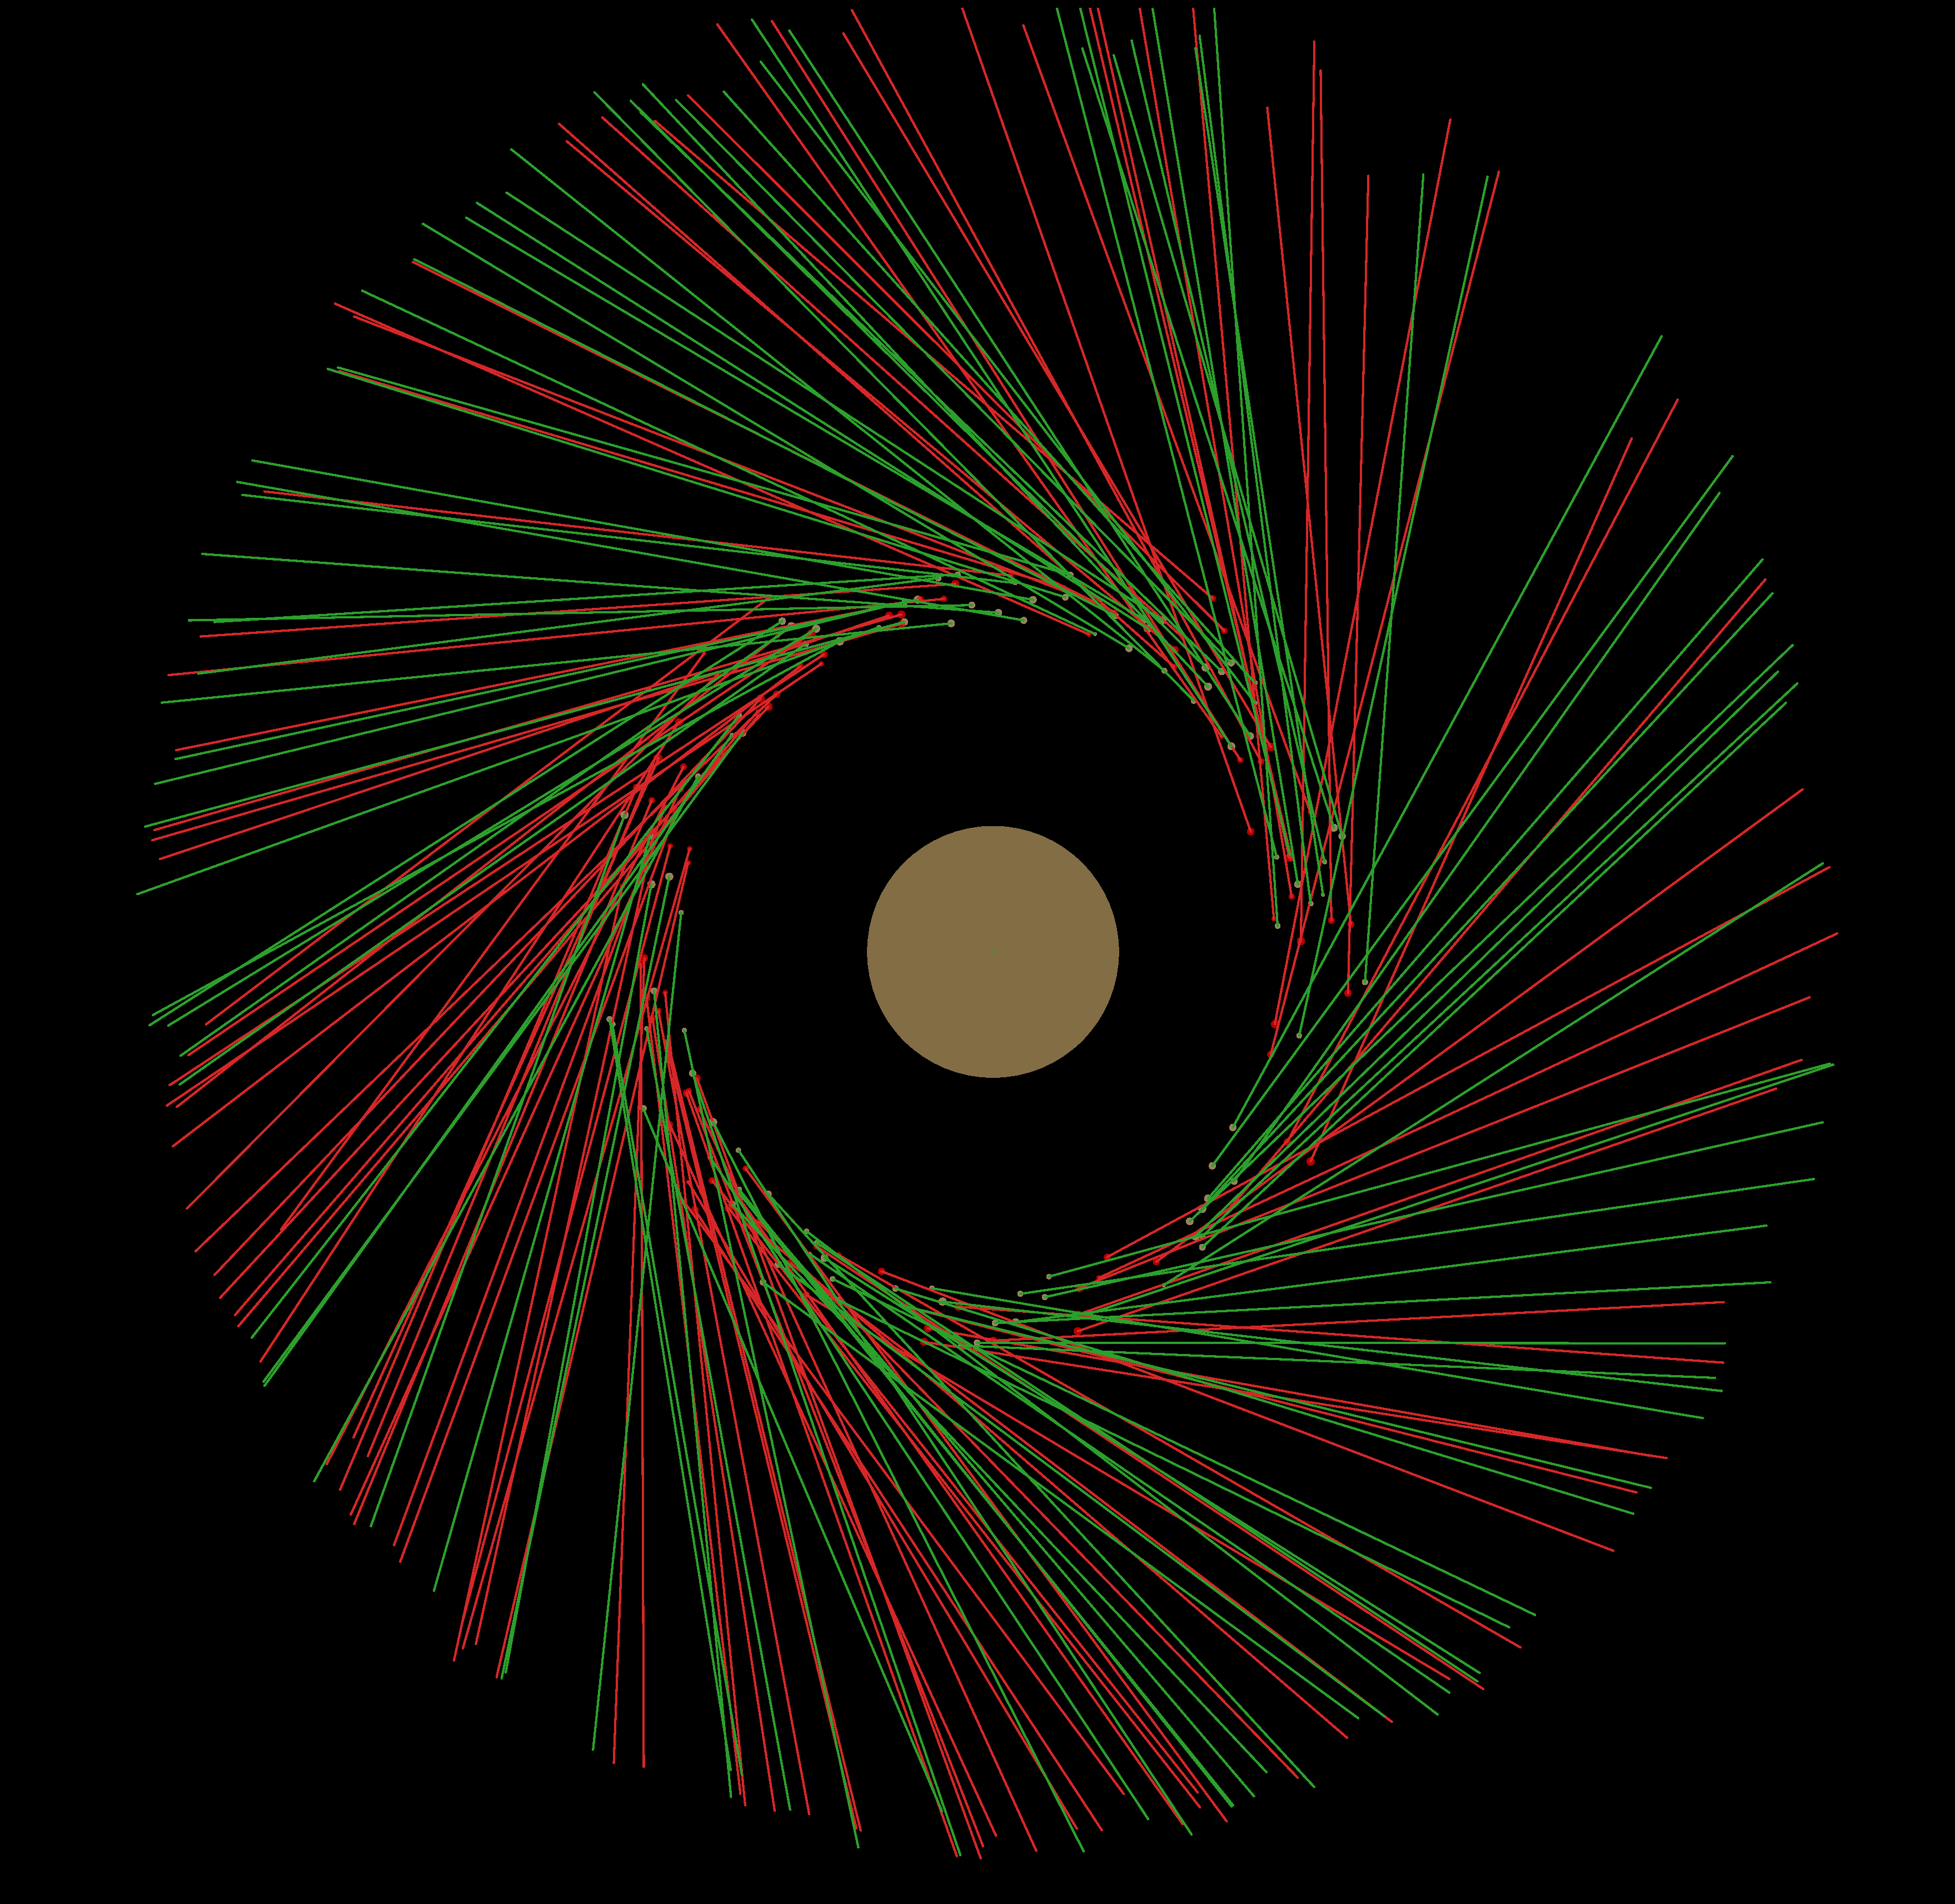
\includegraphics[width=\textwidth]{{img_src/velocity_final_max_100_y_dt_0.0001_y}.pdf}
    \captionof{figure}{The starting and final positions and corresponding velocity vectors of the asteroids with $dt = 0.0001$ years and $t_{max} = 100$ years. The red dots with red lines indicates the final positions and length of the velocity vectors, pointing into their actual directions, while the burly wood color points and green lines are the starting locations and length of the velocity vectors, pointing into the correct directions. The velocities are measured in AU y$^{-1}$ and they are shortened on the graph to the $\frac{100}{8760}$ of their original length.} \label{fig:7}
\end{center}
\vspace*{\fill}